\documentclass[aspectratio=169]{beamer}
\usepackage{amsmath}
\usepackage{tikz}
\usetikzlibrary{angles,quotes,calc}

\title{Starter}
\author{}
\date{}

\setbeamertemplate{navigation symbols}{}

\begin{document}

\begin{frame}
  \frametitle{Starter}

  \begin{columns}[t,onlytextwidth]

    % ===== LEFT COLUMN =====
    \begin{column}{0.4\textwidth}
      % ------------------ Q1 ------------------
      \textbf{1.}


      \vspace{0.7em}
      Which pairs of cardinal directions (North, South, East, West) meet at right angles?

      % ----- Flexible space -----
      \vfill
      \vspace{3em}

      % ------------------ Q3 ------------------
      \textbf{3.}

      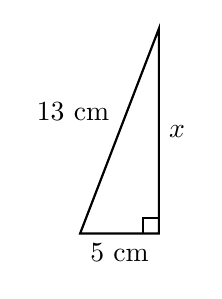
\begin{tikzpicture}[scale=0.2, thick]
        % Right triangle (hypotenuse is 13)
        \coordinate (A) at (0,0);
        \coordinate (B) at (5,0);
        \coordinate (C) at (5,13);

        % Triangle
        \draw (A) -- (B) -- (C) -- cycle;

        % Right angle marker
        \draw ($(B)+(0,1)$) -- ($(B)+(-1,1)$) -- ($(B)+(-1,0)$);

        % Side lengths
        \node[below] at ($(A)!0.5!(B)$) {$5$ cm};
        \node[right] at ($(B)!0.5!(C)$) {$x$};
        \node[above left] at ($(A)!0.5!(C)$) {$13$ cm};

      \end{tikzpicture}

      \vspace{0.5em}
      Find the missing side.

    \end{column}

    % ===== RIGHT COLUMN =====
    \begin{column}{0.6\textwidth}
      % ------------------ Q2 ------------------
      
      \textbf{2.}

      \begin{columns}[t,onlytextwidth]
      \begin{column}{0.5\textwidth}

      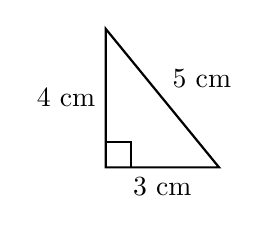
\begin{tikzpicture}[scale=0.8, thick]

        % Coordinates of triangle (hypotenuse longest)
        \coordinate (A) at (0,0);
        \coordinate (B) at (1.8,0);
        \coordinate (C) at (0,2.2);

        % Draw triangle
        \draw (A) -- (B) -- (C) -- cycle;

        % Right angle marker
        \draw ($(A)+(0,0.4)$) -- ($(A)+(0.4,0.4)$) -- ($(A)+(0.4,0)$);

        % Label sides
        \node[below] at ($(A)!0.5!(B)$) {3 cm};
        \node[left]  at ($(A)!0.5!(C)$) {4 cm};
        \node[above right] at ($(B)!0.5!(C)$) {5 cm};

      \end{tikzpicture}
\end{column}
      \begin{column}{0.5\textwidth}
      Which side is the hypotenuse?
\end{column}

    \end{columns}

\textbf{4.}

\begin{columns}[t,onlytextwidth]
  % ===== Diagram Column =====
  \begin{column}{0.45\textwidth}

    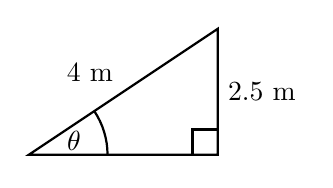
\begin{tikzpicture}[scale=0.8, thick]
      % Triangle for inverse sine
      \coordinate (A) at (0,0);
      \coordinate (B) at (3,0);
      \coordinate (C) at (3,2);

      % Draw triangle
      \draw (A) -- (B) -- (C) -- cycle;

      % Right angle
      \draw ($(B)+(0,0.4)$) -- ($(B)+(-0.4,0.4)$) -- ($(B)+(-0.4,0)$);

      % Side labels
      \node[right] at ($(B)!0.5!(C)$) {$2.5$ m};  % opposite
      \node[above left] at ($(A)!0.5!(C)$) {$4$ m}; % hypotenuse

      % Angle θ at A
      \pic[draw,angle radius=10mm,"$\theta$"{scale=1}] {angle = B--A--C};

    \end{tikzpicture}

  \end{column}

  % ===== Options Column =====
  \begin{column}{0.55\textwidth}

    Find $\theta$.

     \fontsize{10}{12}\selectfont

    \begin{itemize}
        \item[(A)] $\displaystyle \theta = \sin^{-1}\!\left(\frac{2.5}{4}\right)$
        \item[(B)] $\displaystyle \theta = \cos^{-1}\!\left(\frac{2.5}{4}\right)$
        \item[(C)] $\displaystyle \theta = \tan^{-1}\!\left(\frac{2.5}{4}\right)$
    \end{itemize}

  \end{column}
\end{columns}
\end{column}
\end{columns}

\end{frame}

\end{document}
